

% \setcounter{chapter}{1}
\newchapter{Evolutionary Decomposition and the Mechanisms of Cultural Change}{Evolutionary Decomposition and the Mechanisms of Cultural Change}{Evolutionary Decomposition and the Mechanisms of Cultural Change}

\section{Introduction}
   
For the last half-century, many anthropologists and evolutionary biologists have independently realized the fundamental connection between evolutionary theory and cultural change \citep{campbell1965variation, cavalli1981cultural, boyd1985culture, durham1992coevolution, lumsden2005genes, dawkins2006selfish}. Recent decades have witnessed a proliferation of theory regarding the evolution of cultural capacities and traits in humans. Most theorists suppose that culture can be fruitfully studied by imagining it as a set of ``cultural traits," representing socially-learned beliefs and behaviors held by individuals. Cultural evolution, analogous to genetic evolution, occurs when the distribution of these traits changes over time. And as in genetic evolution, we can use mathematical modeling to study the evolutionary mechanisms driving cultural systems. Following this approach, theorists study how natural selection might favor various capacities for social learning, and how these adaptations in turn affect the evolution of behavior and material technology in a population. 

The hypotheses produced by this large theoretical literature have received relatively modest empirical testing, and most of that in controlled, experimental contexts. Many studies have compared the behavior of subjects in multi-armed bandit or cooperation games to models of various social learning strategies \citep{mcelreath2005applying, efferson2007learning, efferson2008conformists, mcelreath2008beyond, mesoudi2008cultural, eriksson2009people, rendell2011copying}. Other task experiments have progressively removed and replaced participants to create multi-generational ``micro-societies" that mimic the development of cultural or technological traditions \citep{baum2004cultural, caldwell2008studying}.  These experiments reveal how various game conditions affect how players learn from others, and how they transmit information through time and space.

As is always the case with experimental studies, it is difficult to evaluate the external validity of this results of these studies.  With a few exceptions \citep{paciotti2003ultimatum, efferson2007learning, chudek2011prestige}, most such experiments use university students, a highly unusual human subgroup \citep{henrich2010weirdest}. Naturalistic studies of real-world cultural phenomena provide a remedy, but quantitative studies of this kind are rare. Most have successfully tested ``static" hypotheses, investigating how ecological and ethnic contexts predict the distribution of cultural beliefs and behaviors at a single point in time \citep{paciotti2003ultimatum, mcelreath2004social, henrich2010evolution, henrich2011nature}. Absent high-resolution longitudinal data, researchers in this theoretical vein can rarely observe cultural change in real-time \citep{gravlee2009methods}. Surely this is due, in part, to the time costs of acquiring such data; evolutionary processes, even cultural ones, are usually long-term and large-scale. Panel studies and historical records provide the most promising avenue for analysis of modern cultural evolution, and in coming years, large-scale data collection and digitization projects will allow access to massive datasets of unprecedented resolution (e.g.~\citealp{michel2011quantitative}).

One major problem facing researchers of cultural evolution is the lack of a principled, quantitative method that can make sense of long-term trends in high-resolution datasets. Consequently, we do not have a firm understanding of how the simplest demographic and evolutionary processes (e.g. differential fertility, survival, individual learning) shape the relative abundance of particular ideas, behaviors or use of technologies.  The best example we know of that analyzes long-term cultural change in an implicitly evolutionary framework is Hout et al.'s \citeyearpar{hout2001demographic} study of the fertility advantages enjoyed by conservative Protestants in the US over the course of the twentieth century. Such demographic work reminds us that the history of a cultural trait is shaped not only by the spread of information from person to person, but also differential migration, birth and death rates.

We argue here that an evolutionary-demographic approach, similar to Hout et al.'s, is the right one for general analyses of cultural evolution. Following the recent work of evolutionary demographers \citep{coulson2008dynamics, ozgul2009dynamics}, we present an equation that decomposes the evolution of any mean character into the contributions of various demographic processes - namely, reproductive success, parent-offspring transmission, death, immigration, individual change, and emigration. We assert that the aggregate of these processes completely describes all evolutionary change; hence, our method provides an exact description of evolution in a cultural system.  With sufficient data, the method may reveal which processes have contributed most to the evolution of any character, which are relatively unimportant, and which ``directions" these processes tend to push.

Our argument proceeds as follows: first, we show mathematically that any change in the mean phenotype of a population of organisms can be decomposed exactly into terms corresponding to standard demographic processes, and argue that these pieces have meaningful evolutionary interpretations. We then decompose the trajectory of a cultural trait from simulated field data into the terms of our equation, which tells us the relative importance of reproductive success, inheritance, death, migration, and individual change to the long term evolution of a hypothetical cultural trait.  Decomposition patterns can also help us model mechanisms underlying a cultural trend, which we demonstrate by fitting various demographic and learning models to the field data to draw tentative conclusions about the major mechanisms underlying the observed cultural evolution.  

\section{The RTDICE Decomposition}

Between any two census times $t$ and $t+1$, the growth of a population of organisms can be calculated using the famous demographer's equation,
\begin{equation} \label{eq:demo}
\Delta N = B - D + I - E
\end{equation}
which decomposes the observed change in population size into four measurable flux quantities, representing the number of births, deaths, immigrants and emigrants, respectively.  Note that although each term clearly represents a distinct demographic process, we cannot consider them strictly in isolation; had the births been greater, the deaths would undoubtedly be different, and so forth.  Moreover, in many realistic situations we can only register deaths among those who had been alive at time $t$, leaving some intercensus events completely inaccessible.  Nevertheless, this decomposition equation gives a clear sense of both \textit{how much} the population is changing and, to some extent, \textit{why}.  Population growth due to births is different than growth through immigration by the same amount, and distinguishing between them is vital.  Our analysis begins by asking whether a similar decomposition can be done for the evolutionary trajectory of a phenotypic trait measured on the population.

In observing evolution, we require that within each census, each individual $i$ possesses some observable phenotypic value, $\phi_i$.  This may represent their ethnicity, age, height, athletic ability, income, religion, occupation, number of livestock owned, political opinions, consumer preferences, or any other quantifiable trait whose population properties we care to track.  Since we leave the phenotype unspecified, this analysis applies to any species of organism, though we will focus here on tracking human phenotypic trajectories.  Given this goal, we seek a decomposition equation for the intercensus change in the \textit{mean phenotype} of the population, $\overline{\phi}$, analogous to Equation \ref{eq:demo}.  Below we present the derivation for one such equation, the RTDICE decomposition.\footnote{RTDICE stands for ``reproduction, transmission, death, immigration, change, emigration,'' six categories that capture all evolution on the phenotypic distribution.  Here ``change'' means intercensus phenotypic change within individuals.}

For the purpose of exposition, imagine we sum the phenotypic value of every individual in a population at a particular time, such that $\phi = \sum \phi_i$.  We take it as self-evident that this aggregate value can change in only five ways: births and immigrants add their phenotypes, emigrants and deaths subtract theirs, and individuals who remain in the population may change their phenotype between the two periods.\footnote{To be precise, in our analysis all individuals who join the population between time period $t$ and $t+1$ are classified as ``births'' if both their parents were in the population in time $t$, and otherwise are ``immigrants.''  All individuals who were present in the population at time $t$ and left it before $t+1$ are either deaths or emigrants depending on how they left.  With only periodic census data, individuals who both joined and left the population intercensus are invisible to our analysis.}  Thus the aggregate phenotype at the next census, $\phi'$, is given by
	\[\phi' = \phi + \phi_B - \phi_D  + \phi_I + \rho - \phi_E, 
\]
where $\phi_B$ is the sum of phenotypes of intercensus births (as measured at $t+1$), $\phi_D$ of intercensus deaths (using their phenotypes at time $t$), and likewise for immigrants and emigrants.  For those who survived from $t$ to $t+1$, $\rho$ is the sum of the differences between their phenotypes at the two times.  Using Equation \ref{eq:demo}, we can express the population growth ratio (or finite rate of increase) as 
	\[G = N'/N  = 1 + b - d + i - e
\]
where $b=B/N$ is the births between $t$ and $t+1$ per member of the population in time $t$, and so forth for $d$, $i$, and $e$.  Thus, we can write the change in the mean phenotype of the population, $\Delta \overline{\phi} = \overline{\phi}' - \overline{\phi}$, as
	\[\Delta \overline{\phi} = \frac{1}{G}\left(\overline{\phi} + b\overline{\phi}_B - d\overline{\phi}_D + i\overline{\phi}_I + c\overline{\rho} - e\overline{\phi}_E - \overline{\phi}(1 + b - d + i - e)\right).
\]
Let $c=1-d-e$ represent proportion of the population from time $t$ remaining at time $t+1$.  Note that the term $\overline{\phi}_B= \phi_B/B$ represents the mean phenotype among births, $\overline{\phi}_D$ among deaths, and so on.  Rearranging and simplifying gives 
\begin{equation} \label{eq:BDICE}
G \Delta \overline{\phi} =  b(\overline{\phi}_B - \overline{\phi}) - d(\overline{\phi}_D - \overline{\phi}) + i(\overline{\phi}_I - \overline{\phi}) + c \overline{\rho} - e(\overline{\phi}_E - \overline{\phi}).
\end{equation}

Equation \ref{eq:BDICE} decomposes mean phenotypic change as the demographer's equation does for population change.  The first term on the right, $b(\overline{\phi}_B - \overline{\phi})$, can be thought of as the effect of births on mean phenotype, the next term, deaths, then immigration, individual change, and emigration, respectively.  Like the left side of the equation, each term on the right is a product of a rate per capita and a difference.  When applied to census data, Equation \ref{eq:BDICE} allows us to see how births, deaths, migration and individual change separately\footnote{As in the demographer's equation, some intercensus events are often unknown, so these terms are not truly ``independent" in any real population. We clarify this point in the Discussion.} affect the trajectory of mean phenotype.  

Provided parent-offspring relationships are known, we can further decompose the birth term in Equation \ref{eq:BDICE} to distinguish the effect of differential reproductive success of the parents (RS) from the deviation of the child phenotype (transmission bias).  To be specific, the term $\overline{\phi}_B$ can be calculated either by dividing the aggregate of offspring phenotypes by the number of offspring, or expressed using parent phenotypes and a transmission bias term.  If $\delta_k$ represents the difference between the phenotype of each child $k$ and the average phenotype of its parents, then the mean phenotype of births is
	\[\overline{\phi}_B = \frac{1}{bN} \sum^N \frac{f_i}{2} \phi_i + \frac{1}{B} \sum^B \delta_k = \overline{\phi}_{R} + \overline{\delta}.
\]
where $f_i$ is the number of offspring of individual $i$.\footnote{The division by two is necessary for offspring with two parents.}  The term $\overline{\phi}_{R}$ weights parent phenotypes by their reproductive output, while $\overline{\delta}$ captures the difference between offspring and their midparents, on the average.  This distinction provides us the full RTDICE evolutionary decomposition,
\begin{equation}  \label{eq:RTDICE}
G\Delta \overline{\phi} = b(\overline{\phi}_{R} - \overline{\phi}) + b \overline{\delta} - d(\overline{\phi}_D - \overline{\phi}) + i(\overline{\phi}_I - \overline{\phi}) + c \overline{\rho} - e(\overline{\phi}_E - \overline{\phi}).
\end{equation}

As before, the six right-side terms of Equation \ref{eq:RTDICE} decompose the change in mean phenotype into the contributions of differential reproductive success, transmission bias, death, immigration, individual change, and emigration, respectively. 

It is worth recognizing that most of the terms in Equation \ref{eq:RTDICE} can be expressed as covariances (e.g. $d(\overline{\phi}_D - \overline{\phi}) = \cov(d,\phi)$).  This fact immediately reveals the conceptual connection between our demographic decomposition of evolution and the Price equation \citep{price1970selection}.\footnote{Price's famous theorem shows that, in the notation used above, $G \Delta \overline{\phi} = \cov(w, \phi) + G\overline{\delta}$, where $w$ gives the total number of ``descendants'' produced by an individual.  This is the first and most general evolutionary decomposition equation, and is the starting place for what Sean Rice calls the ``algebra of evolution'' \citep{rice2004evolutionary}. If we ignore migration and treat surviving individuals as their own descendants, we recover Price's theorem from our Equation \ref{eq:RTDICE}.}

Equation \ref{eq:RTDICE} is true for any measurable character for any population of a sexually reproducing species (and is easily modified for asexual or unisex populations), and provides insight into the nature of the evolutionary forces at work.  A large magnitude RS term, for example, may indicate the operation of fecundity or sexual selection.  The mortality term could be large or small due to viability selection on the phenotype's distribution.  In a genetic context, transmission bias may indicate mutation or meiotic drive, while individual change gives us knowledge of the role of ontogeny.  For culturally-transmitted phenotypes, both the transmission bias and individual change terms may indicate the presence of learning biases.  Emigration and immigration have less connection to Darwinian forces, but may indicate the importance of dispersal or source-sink effects.  In short, provided we have individual-level data, we can use evolutionary decomposition to profile important trends within data straight away (Table \ref{tab:DemoData} \& \ref{tab:DemoDecomp}).  

		\begin{table}[htbp]
    \begin{center}
    \begin{footnotesize}
    \begin{tabular}{cccc}
    \hline
    \hline
    ID    & Census 1 $\phi_i$ & Census 2 $\phi_i$ & Parents \\
    \hline
    Edward & 1     & \textit{emigrated} &  \\
    Lyn   & 0     & \textit{died}  &  \\
    Pat   & 1     & 0     &  \\
    Susan & 1     & 0     &  \\
    Bob   & 0     & 0     &  \\
    Alex      &   & 1     & Edward, Lyn \\
    Jeff      &   & 0     & Edward, Susan \\
    Mike      &    & 0     & Bob, Pat \\
    Andrew      &  & 1     & (\textit{immigrant})\\
    Ian      &     & 1     & Edward, Susan \\
    \hline
		Mean Phenotype: & 0.6 & 0.375 & \\
		\hline
		
	 	\end{tabular}
	  \caption{A hypothetical dataset with individual-level census data for two time periods, measuring a binary phenotype $\phi_i$ (note that $\phi_i$ can be discrete or continuous in this analysis).  Jeff, Mike, and Ian are born intercensus.  Provided we can identify individuals across multiple time periods and also establish parentage, we can apply Equation \ref{eq:RTDICE} to calculate the decomposition terms for the change in mean phenotype in the population (Table 2).}
		\label{tab:DemoData}
		\end{footnotesize}
		\end{center}
		\end{table}


	\begin{table}[htbp]
  \begin{footnotesize}
  \begin{center}
  \begin{tabular}{lrr}
    
  \textit{Term from Equation \ref{eq:RTDICE}} & \textit{Effect} & \textit{Calculation}\\
  \hline
	Reproductive Success & 0.12	&	$b(\overline{\phi}_{R} - \overline{\phi})$ \\
	Transmission Bias & -0.20	&	$b\overline{\delta}$ \\
	Death & 0.12	&	$-d(\overline{\phi}_D - \overline{\phi})$ \\
	Immigration & 0.08	&	$i(\overline{\phi}_I - \overline{\phi})$\\
	Individual Change &	-0.40	&	$c\overline{\rho}$ \\
	Emigration & -0.08	&	$-e(\overline{\phi}_E - \overline{\phi})$\\
	\hline
	Weighted Mean Change & $1.6 \times -0.225$ &	$G \Delta \overline{\phi}$\\
  
  \end{tabular}%
  \caption{Feeding the data from table 1 into Equation \ref{eq:RTDICE}, we decompose the evolutionary change of -0.225 into the six terms on the right in the above table.  Emigration and immigration effectively cancel each other out, and though individuals with a phenotype value of 1 had more children (positive RS term) and died less (positive mortality term), this is more than offset by the fact their children tend to be phenotype 0's (negative transmission bias).  That, coupled with a unanimous change to phenotype 0 among the three survivors from time $t$, causes the population mean to decrease by 22.5 percentage points.  Because the decomposed terms \textit{must} sum to the observed change under all circumstances, we can ensure the calculations are correct.}
  \label{tab:DemoDecomp}
  \end{center}
  \end{footnotesize}
	\end{table}%
	
	
\section{An Island Simulation: The Rise of Snoobism}

One application of this decomposition analysis is assessing the practical importance of different evolutionary forces. In human cultural evolution, researchers often discuss how beliefs and behaviors can successfully diffuse in multiple ways; vertically, through stable inheritance from parents to offspring, or horizontally/obliquely within a social network \citep{Richerson2005:NBGA}.  As such, when viewing the prevalence of a particular trait over time, we wish to know exactly how much of its trajectory can be attributed to the relative reproductive success of its practitioners, how much to relative horizontal or oblique adoption, and how much to relative migration (e.g.~\citealp{stark1996rise, hout2001demographic}).  Because contrasting evolutionary forces enter Equation \ref{eq:RTDICE} through different terms, we can directly and precisely compare their relative consequences if we have the right data.  

To demonstrate the utility of evolutionary decomposition in profiling important trends in cultural change, we analyze census data generated by an agent-based simulator in the \texttt{R} language, \texttt{SnoobSim}.  Simulations can easily descend into unrealistic omniscience in a virtual world of contrived assumptions.  To avoid this problem, we proceed with two rules: first, everything in the analyzed data must be realistic for researchers to collect in the field, and second, the conclusions drawn must rest purely on the recorded dataset itself, rather than the algorithms that produced the data.  As in real life, the goal is to establish exactly how far we can get without knowing the ``rules'' of the system; it is a feature of our analysis that we can gain much new knowledge about the evolutionary processes behind observed dynamics without knowing their true nature.  

In our simulation, a population of around 1,000 humans arrives in a resource-rich environment akin to Hawaii or New Zealand, and begins growing according to realistic daily mortality and reproduction schedules.\footnote{Individuals within the population reproduce, age and die at age-specific rates comparable to real human populations.  For the technical details of the simulator processes, see the chapter appendix.  The census dataset analyzed here, and R code for \texttt{SnoobSim} are available on the authors' websites.}  Every five years, a full census of the population is collected, recording names, parentage, age, and several phenotypic measures.  After 270 years, the population now numbers about 8,000 individuals and 54 such record tables have been collected, allowing us an extraordinarily high-resolution picture of the population's evolution.

Among the settlers, a minority group adheres to a culturally-transmitted worldview we call Snoobism.  Among other aspects of the belief system, Snoob norms celebrate marrying other Snoobs, having large families of Snoob children, and living a safe, healthy and frugal Snoob lifestyle.  Purely for simplicity, we treat this as a discrete, binary trait individuals may acquire or lose in the course of their lifetimes.  Encompassing around a fifth of the original settlers, Snoobism spreads to nearly every member of the population by the final census, twelve generations later.  

Following Ozgul, et al.~\citeyearpar{ozgul2009dynamics}, we contend that evolutionary decomposition can provide a uniquely straightforward understanding of this trend.  If we plug the records of each of the 54 censuses into the RTDICE equation, we produce decomposition terms for each of the 53 values of $\Delta \overline{\phi}$, as in Table \ref{tab:DemoDecomp}.  This information is collected and organized in Figure \ref{fig:Snoob}.

\begin{figure}[t]
\begin{center} 
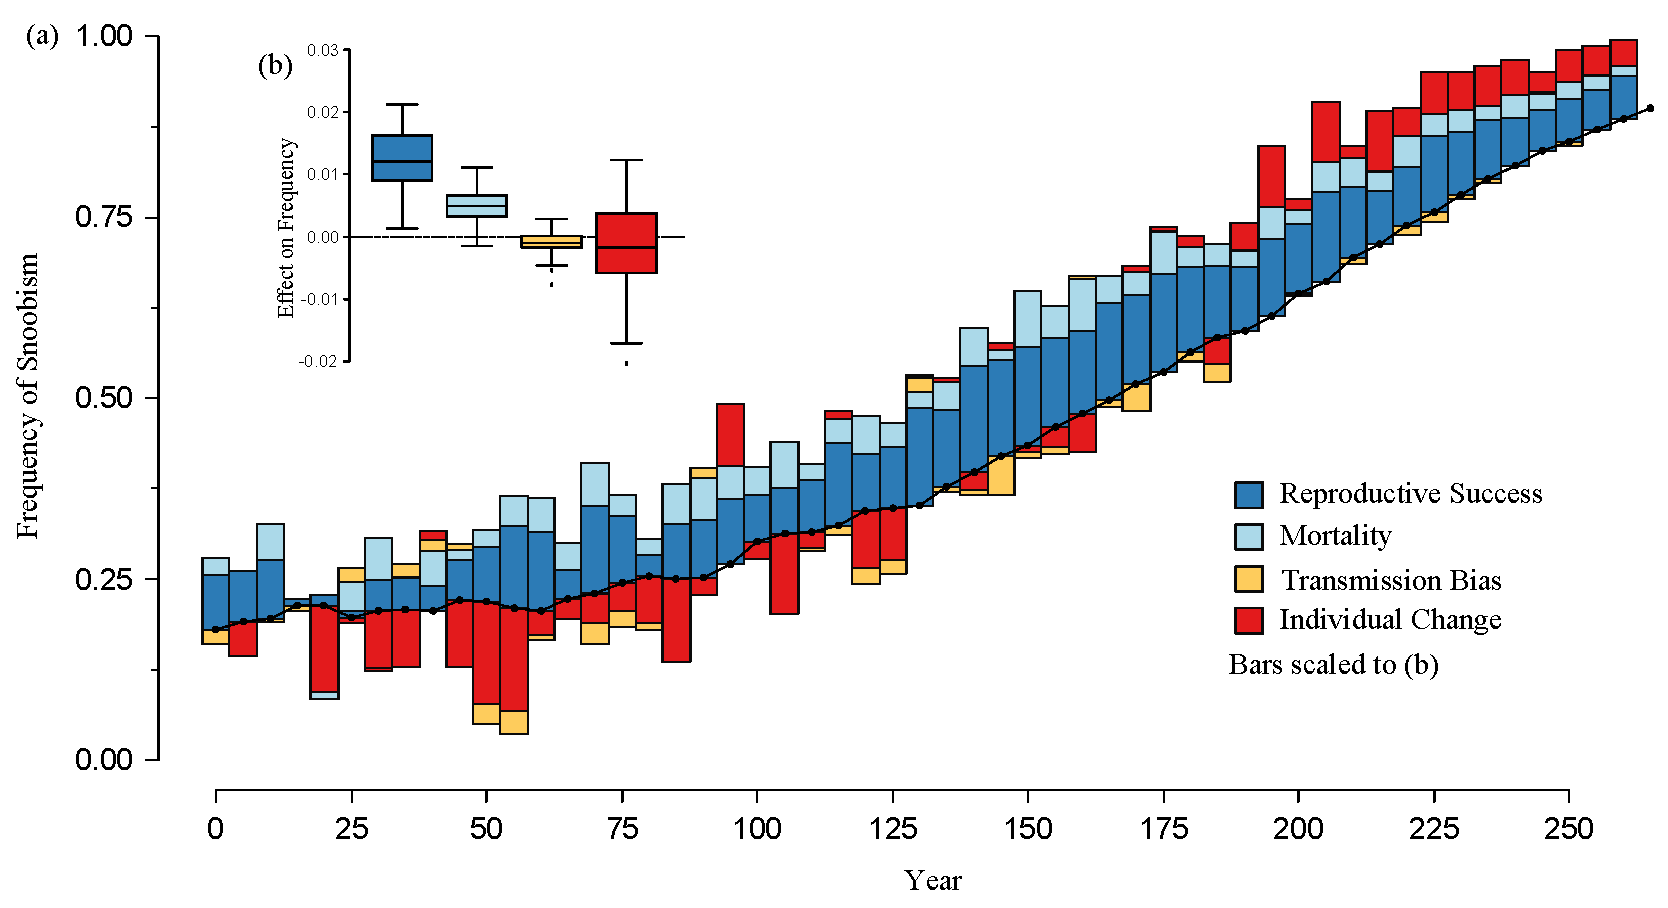
\includegraphics[scale=0.5]{figures/rtdice/FigSnoobCol.pdf}
\caption{(a) The population frequency of a binary cultural trait, Snoobism, observed over time, superimposed with the nonzero decomposition terms from the RTDICE equation.  Bars stacked above the Snoob frequency line represent positive magnitudes, and stacked below it, negative.  Since each bar represents one of the terms of Equation \ref{eq:RTDICE} (divided by $G$), their sum steers the direction of the frequency line.  For clarity, the bars are exaggerated to the scale in (b), which shows means, 5th, 25th, 75th and 95th percentiles of the observed annual decomposition magnitudes for each term.}
\label{fig:Snoob}
\end{center}
\end{figure}

Displaying each of the RTDICE magnitudes and directions graphically over time (Figure 1a) and in summary (Figure 1b) tells us immediately which of the decomposition terms played the largest role in driving the observed cultural trend.  For nearly three centuries, RS and mortality have consistently positive demographic effects on Snoobism, while parent-offspring transmission bias is small and apparently nondirectional.  Note that from the RTDICE decomposition itself we cannot tell if this RS effect results from differences in birth spacing, length of reproductive career, success in acquiring mates, or some combination of these.  Whatever the case, though, it is clear that on average Snoobs have more children than non-Snoobs, and that this is the most important trend in the evolution of Snoobism in the population over time.  

The strong, consistently positive effects from RS and mortality are not obvious from the frequency line itself, which for a full century shows little change in the prevalence of Snoobism in the population.  The decomposition terms indicate the reason: despite the fact the average Snoob has more children and is less likely to die than a non-Snoob, many more individuals abandon Snoobism than adopt it, maintaining Snoob frequency at around 20-25\%.  Only once this effect begins to vanish, 100 years after the settlement's founding, does Snoobism increase in frequency, and the last 15 census records all indicate a positive conversion balance that rivals the RS and mortality effects and facilitates Snoobism's eventual dominance.  

As with differential fertility and mortality, this reversal is consistent with many hypotheses. For example, it could be that an environmental or social change occurred some time between the years 130 and 180, after which Snoobism appeared to be an inherently more attractive lifestyle. Perhaps Snoobs developed a new institution for promoting conversion or preventing apostasy, or became politically dominant over non-Snoobs.  The trend is also consistent with a social learning hypothesis. Suppose, for example, that individuals tend to conform to the beliefs of the majority; then we would expect the conversion balance to covary with $\overline{\phi}$.  In our view, evolutionary decomposition is most valuable because such revealed trends can motivate targeted statistical modeling, which in turn can make predictions about future change.  

From the decomposition figures, we can also clearly see which processes \textit{don't} have large impact on the evolutionary trajectory. If we were measuring traits that are mostly transmitted horizontally within cohorts, such as musical preferences or use of a new technology, we expect to see a large transmission bias between parents and children.  This will also occur when measuring a life history characteristic like body weight or hunting skill, and as we discuss later this may even motivate a more sophisticated decomposition equation. The small bars of the transmission bias term in Figure 1 show that this is not true for one's Snoob status - children, when first censused, reliably hold the traits of their parents, Snoob or non-Snoob.

It should be noted that the apparent lack of a strong transmission bias does not render the process of character transmission unimportant. The fact that offspring tend to resemble their parents on average suggests that the Snoob trait is somehow heritable, and this heritability allows differential fertility and survival to affect the population mean. Still, Figure \ref{fig:Snoob} clearly shows that transmission bias in and of itself appears to have little direct effect on the rise of Snoobism, while the mechanisms behind RS, mortality and individual change all play determining roles.  


\section{Comparing Mechanisms of Cultural Change}

With decomposed trends now available, researchers can make informed forecasts about future change, compare parallel trends for other traits or in other populations, or design more specific goals for new rounds of data collection.  The most useful next step, in our opinion, is generating hypotheses about why these decomposition terms appear as they do, and developing and testing models of the mechanisms underlying these patterns.

For demonstration, we will focus here on the individual change term, with similar analyses of RS and mortality in the chapter appendix.  Among those individuals who appear in multiple censuses, we wish to know what effectively predicts their Snoob status, 0 or 1, at time $t+1$ given the information available at time $t$.  If we consider an individual $i$'s Snoob status in the next census, $\phi_{i,t+1}$, as a binomial random variable, possible mechanisms can be formalized as  conditional probabilities of becoming a Snoob.  To be precise, we will assume individuals retain their current Snoob status with probability $(1-L)$ and update with probability $L$, and using some learning rule $M$.  Then each model takes the form $\Pr(\phi_{i,t+1}=1) = LM + (1-L)\phi_{i,t}$.  As discussed above, the three-century-long swing in direction of the individual change term seems to point to several different, mutually-inclusive mechanisms: 

\textit{Conformist social learning.}  Under this mechanism, individuals tend to abandon Snoobism when it is unpopular, but become Snoobs when it is common.  Beginning with Boyd and Richerson's 1985 model, the conformist learning bias can be expressed in the form $M = \overline{\phi}_t + 2(\beta-1)(2\overline{\phi}_t - 1)\overline{\phi}_t(1-\overline{\phi}_t)$. Parameter $\beta$ represents the strength of conformity; when it is 1, updating is frequency-dependent but unbiased, and when it is greater than 1, updating is biased towards conformity.  More general, but more complicated, versions of this equation have been developed, allowing the conformity threshold to vary from a simple majority \citep{bowles2006microeconomics} and the strength of conformity to vary without bound \citep{mcelreath2008beyond}. 
 
\textit{Individual learning/density dependence.}  As the population is steadily growing in the simulator, the observed swing in the individual change term is also consistent with a simple density-dependence.  Under such a mechanism, the probability of becoming or remaining a Snoob increases with the island's population size, perhaps because non-confrontational Snoob norms are more attractive in crowded environments.  Thus, for population size $N_t$, the updating model may be written as $M=\mathrm{logit}^{-1}(\alpha + \beta N_t)$.  

\textit{Individual learning/environmental change.}  It is also plausible that individuals adopt or maintain Snoobism purely as a consequence of ``environmental'' decision-making, regardless of current population size or Snoob prevalence. Shocks due to technological ratcheting or climatological shifts may make Snoobism, with its thrifty norms and informal channels of social support, a more appealing lifestyle.  The observed swing in the individual change term, then, may be consequent from a changing material environment alone.  Absent any form of economic or ecological data, we can still model this using simple time series models, e.g. $M=\mathrm{logit}^{-1}(\alpha + \beta t)$, which can account for unobserved environmental shifts. 

Of course, in real populations such processes are probably all in effect to varying degrees, so more complex updating models that incorporate mixtures of these simple mechanisms should be included as well.  Using information-theoretic model comparison techniques, we fit a variety of such models, simple and complex, to the individual-level phenotypic data using maximum likelihood, and compared them using the Akaike Information Criterion and Schwartz Criterion (also called BIC).  Table \ref{tab:Learning} shows the four best-performing models, all conformist learning models.  The dominance of such models is most consistent with a pure conformist social learning hypothesis, at least among the few hypotheses tested above.\footnote{Unsurprisingly, this was the learning model used by the agents in \texttt{SnoobSim}.}  The two other major drivers of Snoobism, RS and mortality, were analyzed in a similar fashion in the chapter appendix.  Motivated by patterns in the decomposition terms, hypotheses about driving mechanisms of cultural evolution can be drawn from the rich theoretical literature and, using these methods, fitted to realistic field data.

\begin{table}[htbp]
  \centering
    \begin{footnotesize}
    \begin{tabular}{lccc}
    Updating Model, $M$ & Conformity Coefficient & AIC$_c$ Weight & BIC Weight \\
\hline
\hline
    $\overline{\phi}_t + 2(\beta-1)(2\overline{\phi}_t - 1)\overline{\phi}_t(1-\overline{\phi}_t)$ & 1.366 (1.322, 1.409) & 0.4049 & 0.5010 \\
    $\overline{\phi}_t^{\beta} / (\overline{\phi}_t^{\beta} + (1-\overline{\phi}_t)^{\beta})$ & 1.374 (1.318, 1.429) & 0.4019 & 0.4972 \\
    $\overline{\phi}_t + 2(\beta-1)(2\overline{\phi}_t - 2k)\overline{\phi}_t(1-\overline{\phi}_t)$ & 1.360 (1.311, 1.408) & 0.1743 & 0.0017 \\
    $\mathrm{logit}^{-1}(\alpha + \beta \overline{\phi}_t)$ & 6.389 (6.121, 6.658) & 0.0106 & 0.0001 \\
    \hline
    \end{tabular}%
    \caption{Top four models among the thirteen fitted to the simulated census data, as measured by AIC$_c$ and BIC score (see chapter appendix for full model list).  Each model $M$ of the thirteen is embedded in the equation $p=L(M) + (1-L)(\phi_{i,t})$, where $p$ describes the conditional probability an individual will be a Snoob in the next census, per $\phi_{i, t+1} \sim \mathrm{Binomial}(1, p)$.  The top four are all social learning models, each with a conformity coefficient $\beta$ of comparable meaning.  The first model above comes from Boyd and Richerson (1985), while the second and third come from McElreath, et al. (2008) and Bowles (2004), respectively.} 
		\label{tab:Learning}
    \end{footnotesize}

\end{table}

\newpage
\section{Discussion}

It is important to emphasize what the preceding evolutionary decomposition analysis gives us compared to standard demographic metrics. Birth and death rates could be more precisely compared using the total fertility rate, life expectancy at birth, or other common demographic measures. But by themselves these tools lack a direct mathematical connection to change in mean phenotype in the population, the most common way we measure evolution.  As a result, it is difficult to assess exactly how much mortality affects the population distribution of phenotype, versus RS, immigration, and so forth.  

These answers are readily available from decomposition of mean phenotypic change, regardless of the particularities of the system.  Phenotypes may be discrete values like Snoob status, or continuous, like body weight.  Because the decomposition equation is derived from basic facts about the population and data structure, its value depends not in the realism of its assumptions (which we contend are nearer to axioms), but rather in the meanings we can find in its terms, once strictly defined.  In doing so, three important qualifications must be stressed. 

First, the terms in the decomposition equation segregate but do not correspond exactly to evolutionary processes like sexual selection or biased social learning.  Snoobs may enjoy higher RS because of something inherent in practicing Snoobism, because the trait co-occurs with some other trait like income or age, or simply due to chance. The decomposition terms, most of which are covariances between phenotype and demographic outcomes, are really nothing more that dimensionalized correlations.  Following Rice \citeyearpar{rice2004evolutionary} and Henrich et al. \citeyearpar{Henrich2008:misunderstandings}, we feel that terms like ``selection'' or ``fitness'' should only be invoked when a \textit{causal} pathway between phenotype and outcome can be supported, and even then any empirical decomposition term will be a combination of both causal and noncausal associations. 

Second, the RTDICE decomposition is only one possible partitioning of the observed phenotypic trajectory, and potentially not a very useful one.  For example, the differential mortality between Snoobs and non-Snoobs is partially a consequence of the fact Snoobs tend to be younger, which is a consequence of their differential RS.  We can use logistic models of mortality to establish that Snoob status predicts mortality outcomes even among those of the same age (see chapter appendix), but the RTDICE mortality term cannot isolate this effect from the covariance between Snoobism and age.  If we expect structuring variables like age, gender, ethnic group, or location in a metapopulation will play an important role in the evolution of a particular phenotypic character, we should build this directly into the decomposition equation as appropriate for the dataset and the situation \citep{coulson2008dynamics}.  

We must also modify the equation if the categories we place people within are inappropriate, e.g. the intercensus period spans multiple generations, parentage cannot be identified, or we wish to distinguish immigrants from different sources.  Note that we need no special consideration of whether the parent of record is a genetic parent, and if appropriate we may specify other inheritance relationships like ``teacher'' or ``older sibling''; the evolutionary consequences of the observed relationship are an empirical matter.

The third qualification is that, without records of each demographic event as it happened, the terms in a decomposition equation should not be viewed as strictly independent.  The effects of intercensus events are inferred from comparing the two census records, but some information is necessarily lost, such as individual change shortly before death or after birth. 

In fact, if the population experiences demographic events in discrete seasons, the terms can lose their distinctiveness altogether.  Imagine, for example, a population of individuals experience heavy mortality in each winter, selecting out individuals with smaller phenotypes (e.g. weight, beak length).  Then, in the summer, the survivors give birth.  Applying RTDICE to annual census records would show a strong covariance between RS and phenotype even if phenotype plays no important role in mating or reproducing, simply because of the preceeding mortality event.  

We suspect that for large populations in which such demographic events do not follow a strict order, the distortions are minimal.  We can never properly rid ourselves of the problem of order, however, since every death removes the possibility of another birth, emigration event, etc.  For populations which do go through a distinct schedule of demographic events, one possible solution is to construct ordered-event decomposition equations.  

As in Coulson and Tuljapurkar \citeyearpar{coulson2008dynamics}, the RTDICE equation only holds exactly for full census data without error. We realize that probably no dataset of the size and quality comparable to that simulated here exists in reality; real datasets nearly always contain just a sample of the full population and some amount of measurement error. Under circumstances of incomplete data, the terms of the RTDICE equation cannot simply be computed but must instead be estimated by statistical analysis. We anticipate that future research will elucidate the best statistical methods for estimating these terms.

Despite these limitations, we foresee a wide variety of applications for the decomposition approach in both evolutionary theory and studying human history.  The decomposition method provides unique advantages in profiling trends, motivating and testing hypotheses, and assisting prediction.  By applying basic demographic bookkeeping to high-resolution records of cultural change over time, we are also able to demonstrate conclusively the Darwinian nature of cultural transmission.    





\section{Appendix to Chapter 2}

All models below were coded in R using variables extracted from the 54 SnoobSim census records.  Models were fit by maximum likelihood using the function \texttt{mle2} in Ben Bolker's \texttt{bbmle} package (cran.r-project.org/), with the default BFGS algorithm.

\subsection{Extended Analysis of Individual Change}

The ``individual change'' decomposition bars indicate that initially the balance of change is negative and large in magnitude.  As the frequency of Snoobs approaches 50\%, though, this effect becomes smaller and smaller, and as Snoobs move towards fixation the effect reverses and the balance of converts is now strongly positive, at times rivaling RS in magnitude.

An important thing to keep in mind when reading the individual change bars is that they represent only the average phenotypic cange across individuals; some individuals became Snoobs in the first few decades, but more apostatised to non-Snoob.  

Our outcome variable here is ``will be a Snoob'' in the next census ($\phi_{i,t+1}$), modeled by current Snoob status and other properties of individuals and the population.  Because we have a binary outcome variable, we use a binomial model with various parameterizations of $p$.  A standard way to express this probability is the form $p = LM + (1-L)\phi_{i,t}$, so individuals update with probability $L$ and retain their current status with probability $(1-L)$.  Strictly speaking, this sequence of first updating, then (potentially) changing phenotype implied by this model is quite artificial for real human learning.  However, it is interesting to consider human cultural change \textit{as if} it proceeded in this fashion, because the updating rule can incorporate a variety of hypothesized mechanisms for comparison using information criteria. 

The simplest model is a constant Snoob conversion probability for all individuals
	\[M_0 = \alpha.
\]
In other words, individuals update with probability $L$, and of those we expect fraction $\alpha$ take Snoobism as their phenotype.

Conformist learning is parameterized in four, very similar, ways.  The model $\overline{\phi}_t + D(2\overline{\phi}_t-1) \overline{\phi}_t (1-\overline{\phi}_t)$ is from \cite{boyd1985culture}.  Parameter $D$ represents the strength of conformity; $D=0$ indicates no conformity and unbiased, frequency-dependent learning.  If $D > 0$, conformity will increasingly dominate the probability of becoming a Snoob, while $D < 0$ implies non-conformity (you are more likely to choose the opposite of the majority's trait).  Bowles \cite{bowles2006microeconomics} modifies this by creating an explicit parameter for the threshold, allowing it to vary from 0.5, so which we could write as $\overline{\phi}_t + D(2\overline{\phi}_t-2k)\overline{\phi}_t(1-\overline{\phi}_t)$.  The conformity model in McElreath, et al. \citep{mcelreath2008beyond}\footnote{The basic form of this model was suggested to McElreath et al. by Sam Bowles (Richard McElreath, \textit{personal communication}).} expresses a similar idea, using the model
	\[ M_1 = \frac{\overline{\phi}_t^\beta}{\overline{\phi}_t^\beta + (1-\overline{\phi}_t)^\beta}
\]
where $\beta > 1$ represents conformity.  Because the Boyd and Richerson model is actually Taylor series approximation of this more general model when $\beta$ is close to 1 and $\overline{\phi}_t$ is near 0.5, we may sensibly write all three models in a common notation.  Hence, in our analysis, we include the 1985 model as
	\[ M_2 = \overline{\phi}_t + 2(\beta-1)(2\overline{\phi}_t-1),
\]
and the 2004 model as
	\[ M_3 = \overline{\phi}_t + 2(\beta-1)(2\overline{\phi}_t-2k).
\]
Another sensible way to parameterize conformity is by using a logit link function, such that
	\[ M_4 = \mathrm{logit}^{-1}(\alpha + \beta \overline{\phi}_t) = \frac{\exp(\alpha + \beta \overline{\phi}_t)}{1 + \exp(\alpha + \beta \overline{\phi}_t)}. \]

Two density-dependent models, one with a quadratic effect,
	\[ M_5 = \mathrm{logit}^{-1}(\alpha + \beta N_t),\]
	\[ M_6 = \mathrm{logit}^{-1}(\alpha + \beta_1 N_t + \beta_2 N_t^2).\]
Model $M_6$ used population sizes coded in standard units, to aid the maximum likelihood algorithm. Two time series models, one with a quadratic effect,
	\[ M_7 = \mathrm{logit}^{-1}(\alpha + \beta t),\]
	\[ M_8 = \mathrm{logit}^{-1}(\alpha + \beta_1 t + \beta_2 t^2 ).\]
Oscillatory models of time and population were also used:
	\[ M_9 = \mathrm{logit}^{-1}(\alpha + \beta_1 \sin (\beta_2 t)),\]
	\[ M_{10} = \mathrm{logit}^{-1}(\alpha + \beta_1 \sin (\beta_2 N_t)).\]
Various combinations were also included.  Including time and population size,
\[ M_{11} = \mathrm{logit}^{-1}(\alpha + \beta_1 t + \beta_2 N_t).\]
Including population Snoob frequency, individual age in years (centered on mean), and gender (coded as a 1/0 variable ``male''),
\[ M_{12} = \mathrm{logit}^{-1}(\alpha + \beta_1 \overline{\phi}_t + \beta_2 \mathrm{male} + \beta_3 \mathrm{age}).\]
The final model included adds time to model $M_{12}$,
\[ M_{13} = \mathrm{logit}^{-1}(\alpha + \beta_1 \overline{\phi}_t + \beta_2 \mathrm{male} + \beta_3 \mathrm{age} + \beta_4 t).\]
Running a model comparison ranks these thirteen models according to Table \ref{tab:ichangemodels}.  Schwartz criterion ranks (BIC) are nearly identical to AIC$_c$ ranks, nominating models $M_1$ and $M_2$ as the best-performing.  The constant model, $M_0$, performs worst among the model set, but conformity models completely dominate the model weighting.  This would indicate that the best out-of-sample predictive models as identified by information theory are purely social learning models using $\overline{\phi}_t$, and do not improve by adding other population-level covariates like population size, or individual-level variables like gender or age.

 
\begin{table}[htbp]
  \centering
    \begin{tabular}{lrrrrr}
  	\hline
  	\hline
    Model & $k$ & AIC$_c$ weight & BIC weight & $\Delta$ AIC$_c$ & $\Delta$ BIC \\
   	\hline
    $M_2$  & 2     & 40.49\% & 50.10\% & $<$0.01  & $<$0.01 \\
    $M_1$  & 2     & 40.19\% & 49.72\% & 0.02  & 0.02 \\
    $M_3$  & 3     & 17.44\% & 0.17\% & 1.69  & 11.42 \\
    $M_4$  & 3     & 1.06\% & 0.01\% & 7.28  & 17.02 \\
    $M_{12}$ & 5     & 0.58\% & $<$0.01\% & 8.48  & 37.68 \\
    $M_{13}$ & 6     & 0.24\% & $<$0.01\% & 10.27 & 49.21 \\
    $M_6$  & 4     & $<$0.01\% & $<$0.01\% & 67.35 & 86.82 \\
    $M_8$  & 4     & $<$0.01\% & $<$0.01\% & 102.91 & 122.38 \\
    $M_7$  & 3     & $<$0.01\% & $<$0.01\% & 107.40 & 117.14 \\
    $M_5$  & 3     & $<$0.01\% & $<$0.01\% & 921.84 & 931.57 \\
    $M_{11}$ & 4     & $<$0.01\% & $<$0.01\% & 1070.58 & 1090.05 \\
    $M_{10}$ & 4     & $<$0.01\% & $<$0.01\% & 2007.97 & 2027.44 \\
    $M_9$  & 4     & $<$0.01\% & $<$0.01\% & 2254.17 & 2273.64 \\
    $M_0$  & 1     & $<$0.01\% & $<$0.01\% & 133107.95 & 133098.21 \\
    \hline
    \end{tabular}%
    \caption{Individual change updating models, by AIC$_c$ rank, with AIC$_c$ and BIC scores in terms of the top model, $M_2$, and model weights (all to two decimal places).  Both the Akaike Information Criterion and the Schwartz Criterion (BIC) rank the performance of each model by assigning penalties to its MLE likelihood value; AIC and AIC$_c$ penalize by the number of parameters, $k$, in a given model.}
  \label{tab:ichangemodels}%
\end{table}%

Because of the functional similarity between $M_1$, $M_2$, and $M_3$, the parameter estimates are nearly identical, and only $M_1$ will be discussed.  The conformity coefficient (with standard error) was estimated as 1.374 (0.028), which, being above 1, is evidence towards conformist biased updating.  The maximum-likelihood estimate for the intercensus updating probability, $L$, was 0.100 (0.002), meaning that under this model about 10\% of the population updates every five years, while 90\% do not update at all.  It is worth noting these estimates are quite sensible per what the SnoobSim software is actually doing (next section).

\begin{figure}[t]
\begin{center}
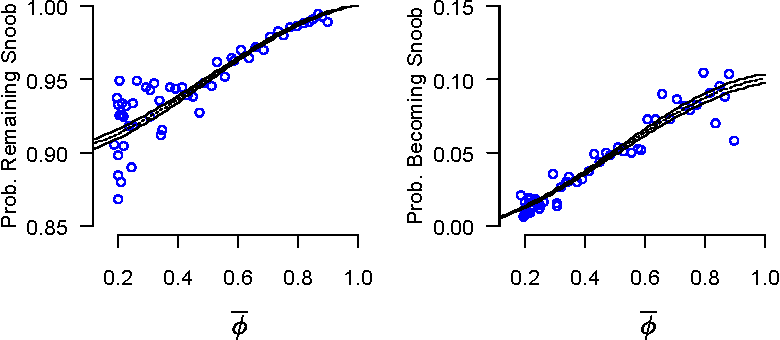
\includegraphics[scale=1]{figures/rtdice/ichange.pdf}
\caption{Fitted model $M_1$ plotted over the observed proportions of individuals who will switch to or remain Snoobs intercensus, on the population Snoob frequency for the first 53 censuses.  Maximum likelihood estimates (dashed line) and 95\% HPDI intervals (solid lines) for the Bernoulli probability of becoming a Snoob, $p$, show a strong nonlinear association between individual change and $\overline{\phi}_t$.}
\label{fig:ichange}
\end{center}
\end{figure}


\subsubsection{Individual Change - What SnoobSim is Actually Doing}

In the simulation, each day, some fraction of the population decides they will ``update'' their Snoob status.  To be precise, each individual updates daily with probability 0.00006.  If an individual decides to update, they then collect a random sample of 100 people in the population, and uses this information to decide to change their Snoob status or stay where they are.  Note that once an individual decides to update, their previous Snoob status becomes irrelevant.  Each individual takes their particular sample of 100 and adopts Snoobism with probability given by the code:

\begin{verbatim}
prob.converting.to.snoob <- 
	(sample.frq^conformity.bias.snoob)/
	(sample.frq^conformity.bias.snoob	+ (1-sample.frq)^conformity.bias.snoob)
\end{verbatim}

In other words, learners used exactly the same mechanism as $M_1$, except on the Snoob frequency among the 100 they randomly sampled, rather than the population frequency.  No surprise, then, that models with this functional form came in first in the model comparison.  The simulation parameter \texttt{conformity.bias.snoob} was set to 1.3 (compare against the MLE of $\beta$ above), and with a daily probability of updating set to 0.00006, we expect proportion $1-(1-0.00006)^{365\times5}=0.104$ of the population to update (compare to the MLE of $L$, above).  We should not expect real census data to nominate such simple models, but the utility of information-theoretic model comparison remains the same nonetheless.


\subsection{Analysis of RS Term}

The strong, consistently positive effect of RS in the decomposition indicates that Snoobs have more children than non-Snoobs, on the average.  This could be causal, meaning Snoobism itself may have some effect on one's desire or ability to mate, or it could be a consequence of Snoobism covarying with some other trait.  For example, if people tend to become Snoobs during their reproductive careers, only to abandon it later in life, we would see a consistent, positive effect in the decomposition.  Or, perhaps Snoobism is a sex-specific trait and there are fewer of that gender in the population (so they must have higher mean RS).  

Hence, it is premature to say Snoobism is ``under selection'' without conclusive evidence against confounding variables.  This is difficult to impossible in observational contexts, like this one, but statistical control can at least tell us if the RS advantage of Snoobs remains when comparing Snoobs and non-Snoobs of the same gender and age.  

Our outcome variable is the number of kids an individual sires (if they are of reproductive age) have during the next intercensus period, which in our data varies between 0 and 8 (women are constrained to about 5 or 6 children in a five-year intercensus period), $f_{i, t+1}$.  We have some flexibility with count data, so we have chosen to compare models of the outcome variable using three possible probability distributions: geometric, Poisson, and zero-inflated Poisson.  For the Poisson family, $\lambda$ is modeled by an exponential link function ($\lambda = \exp(M)$, for some model $M$), while for the geometric models, the Bernoulli probability of success $p$ is modeled generically by logit link function ($p=\mathrm{logit}^{-1}(M)$).  

Altogether, twelve models of the expected number of intercensus children were compared.  Note that all uses of age center the variable on its mean.
	\[M_0 = \beta_0
\]
	\[M_1 = \beta_0 + \beta_1 \mathrm{age}
\]
	\[M_2 = \beta_0 + \beta_1 \mathrm{age} + \beta_2 \mathrm{(age)}^2
\]
	\[M_3 = \beta_0 + \beta_1 \mathrm{age} + \beta_2 \mathrm{(age)}^2 + \beta_3 \phi_{i,t}
\]
	\[M_4 = \beta_0 + \beta_1 \mathrm{age} + \beta_2 \mathrm{(age)}^2 + \beta_3 \phi_{i,t} + \beta_4 \mathrm{male}
\]
	\[M_5 = (1-N_t/K)(\beta_0 + \beta_1 \mathrm{age} + \beta_2 \mathrm{(age)}^2 + \beta_3 \phi_{i,t} + \beta_4 \mathrm{male})
\]
	\[M_6 = \exp(-K*N_t)(\beta_0 + \beta_1 \mathrm{age} + \beta_2 \mathrm{(age)}^2 + \beta_3 \phi_{i,t} + \beta_4 \mathrm{male})
\]
	\[M_7 = \beta_0 + \beta_1 \mathrm{age} + \beta_2 \overline{\phi}_t
\]
	\[M_8 = \beta_0 + \beta_1 \mathrm{age} + \beta_2 \mathrm{(age)}^2 + \beta_3 \overline{\phi}_t
\]
	\[M_9 = \beta_0 + \beta_1 \mathrm{age} + \beta_2 \mathrm{(age)}^2 + \beta_3 \phi_{i,t} + \beta_4 \overline{\phi}_t
\]
	\[M_{10} = \beta_0 + \beta_1 \mathrm{age} + \beta_2 \mathrm{(age)}^2 + \beta_3 \phi_{i,t} + \beta_4 \mathrm{male} + \beta_5 \overline{\phi}_t
\]
	\[M_{11} = \beta_0 + \beta_1 \mathrm{age} + \beta_2 \mathrm{(age)}^2 + \beta_3 \phi_{i,t} + \beta_4 \mathrm{male} + \beta_5 (\mathrm{male} \times \phi_{i,t})
\]
	\[M_{12} = \beta_0 + \beta_1 \mathrm{age} + \beta_2 \mathrm{(age)}^2 + \beta_3 \phi_{i,t} + \beta_4 \mathrm{male} + \beta_5 \overline{\phi}_t + \beta_6 (\mathrm{male} \times \phi_{i,t})
\]
Since each of these 12 models can be placed within a Poisson, geometric, or zero-inflated Poisson (ZIP) distribution, a total of 36 distinct models are fitted separately to the data and compared for out-of-sample predictive accuracy using AIC$_c$ and BIC (Table \ref{tab:RScompare}).

The top models, $M_{10}$ and $M_{12}$, both include age, gender and Snoob status, and differ only in an interaction effect between male and Snoob status.  No density-dependent or frequency-dependent models performed as well.  Also, according to the model comparison, the zero-inflated Poisson distribution is the best-performing stochastic wrapper around these two models, as opposed to the geometric distribution or the Poisson, which are vastly outperformed.

Estimates and confidence intervals for $M_{10}$ are presented in table \ref{tab:m10ests}, with MLE-fitted lines plotted in Figure \ref{fig:rs}.  It is clear from the estimates and figure that Snoobism remains an excellent predictor of reproductive output after accounting for age and gender.  This allows us to rule out the possibility that the decomposition results for RS were merely a consequence of chance associations between Snoobism and age or gender, and points to the possibility Snoobism is under some form of fecundity or sexual selection.    

\begin{table}[htbp]
  \centering
    \begin{tabular}{lcrrrr}
    \hline
    \hline
    Parameter & Estimate & Std. Error & 2.50\% & 97.50\% \\
    \hline
    $\beta_0$    & -0.878 & 0.024 & -0.924 & -0.831 \\
    $\beta_1$    & -0.006 & $<$0.001 & -0.007 & -0.005 \\
    $\beta_2$    & -0.002 & $<$0.001 & -0.003 & -0.002 \\
    $\beta_3$    & 0.681 & 0.017 & 0.647 & 0.714 \\
    $\beta_4$    & 0.120 & 0.013 & 0.093 & 0.147 \\
    $\beta_5$    & 0.244 & 0.033 & 0.179 & 0.309 \\
    $\alpha$ & 0.357 & 0.006 & 0.3451 & 0.369 \\
    \hline
    \end{tabular}%
    \caption{Parameter estimates for the zero-inflated Poisson version of model $M_{10}$.  The second-placed model's fitted values are nearly identical to these but with an additional interaction term for Male snoobs of -0.043 (0.030), MLE and SE.  Parameter $\alpha$ estimates the frequency an outcome of 0 will be drawn from the distribution, beyond what would be expected by the Poisson model.} 
  \label{tab:m10ests}%
\end{table}%

\begin{table}[htbp]
  \centering
    \begin{tabular}{llrrrrr}
    \hline
    \hline
    Model & Distribution & $k$ & AIC$_c$ weight & BIC weight & $\Delta$ AIC$_c$ & $\Delta$ BIC \\
    \hline
    $M_{10}$ & ZIP   & 7     & 72.35\% & 99.63\% & 0.00  & 0.00 \\
    $M_{12}$ & ZIP   & 8     & 27.65\% & 0.37\% & 1.92  & 11.17 \\
    $M_{12}$ & Geom. & 7     & 0.00\% & 0.00\% & 28.19 & 28.19 \\
    $M_{10}$ & Geom. & 6     & 0.00\% & 0.00\% & 36.98 & 27.73 \\
    $M_4$  & ZIP   & 6     & 0.00\% & 0.00\% & 52.23 & 42.98 \\
    $M_{11}$ & ZIP   & 7     & 0.00\% & 0.00\% & 53.70 & 53.70 \\
    $M_{11}$ & Geom. & 6     & 0.00\% & 0.00\% & 72.55 & 63.30 \\
    $M_{4}$ & Geom. & 5     & 0.00\% & 0.00\% & 80.50 & 62.00 \\
    $M_3$  & Geom. & 4     & 0.00\% & 0.00\% & 98.63 & 70.87 \\
    $M_3$  & ZIP   & 5     & 0.00\% & 0.00\% & 129.07 & 110.57 \\
    $M_8$  & Geom. & 4     & 0.00\% & 0.00\% & 1553.27 & 1525.52 \\
    $M_8$  & ZIP   & 5     & 0.00\% & 0.00\% & 1699.65 & 1681.15 \\
    $M_{12}$ & Poisson & 7     & 0.00\% & 0.00\% & 1779.76 & 1779.76 \\
    $M_{10}$ & Poisson & 6     & 0.00\% & 0.00\% & 1795.46 & 1786.21 \\
    \hline
    \end{tabular}%
    \caption{Models of reproductive success, by AIC$_c$ and BIC rankings to two decimal places.  Models can appear more than once in the rankings because they are embedded in different stochastic nodes: the second-ranked model is $M_{12}$ in a zero-inflated Poisson distribution (ZIP), while the third-ranked model is $M_{12}$ in a geometric distribution.  Of the 36 models tested (three stochastic distributions for each of twelve structural models), only the top 14 are shown.}
  \label{tab:RScompare}%
\end{table}%


\begin{figure}[t]
\begin{center}
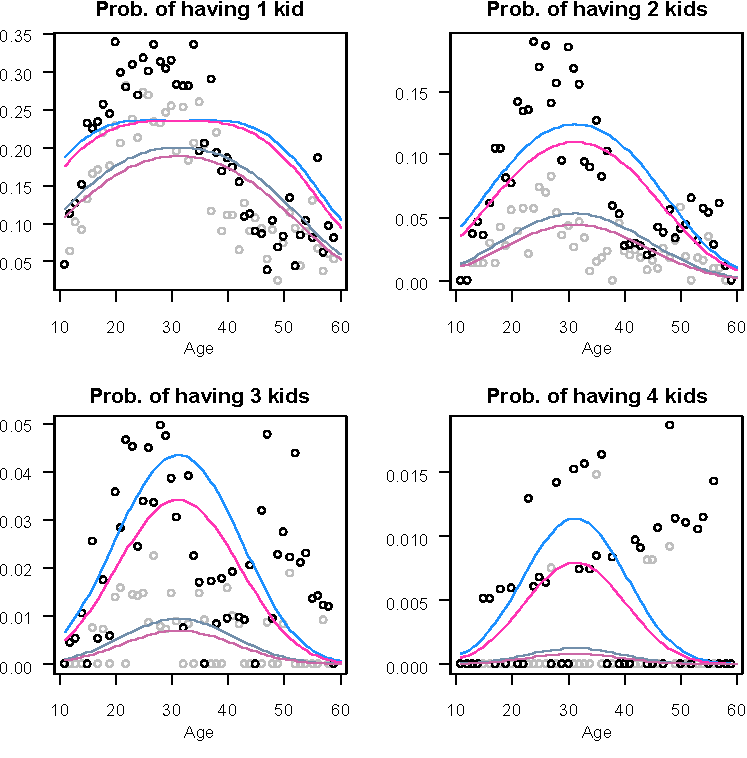
\includegraphics[scale=1]{figures/rtdice/rs.pdf}
\caption{Fitted model $M_{10}$ plotted over the observed proportions of parents with exactly a certain number of intercensus children, by parent age.  For each of the 53 intercensus periods, Snoobs (black circles) have more children on average than non-Snoobs (gray circles), which reflected by the fitted lines as well.  Snoob men (bright blue) have more children on average than both Snoob women (bright pink) and non-Snoob men (dark blue), implying a sex-ratio imbalance.}
\label{fig:rs}
\end{center}
\end{figure}


\subsubsection{Reproductive Success: What SnoobSim is Actually Doing}

Women become pregnant probabilistically according to an age-specific fertility schedule identical to that of a realistic population (US women c. 2005).  From the ages of 15 to 50, women reference a daily probability of conception given by

\begin{verbatim}
daily.pr.conception <- (1-(1/(1+exp(alpha + beta1*snoob))))
\end{verbatim}

Parameter \texttt{alpha} is set by the fertility schedule, and the effect of being a Snoob is for this run is \texttt{beta1}=0.8, exaggerating a Snoob's age-specific fertility schedule and increasing the daily probability she will become pregnant.  If a woman conceives, she will then choose a male as the father.  

Men are promiscuous and can be chosen by multiple women (one lucky man fathered a record 8 kids in 5 years with several different women).  Women will continue to mate with the same man until he becomes unavailable due to advanced age (i.e. greater than 60 years old) or death.

According to the simulator parameters, women almost always choose males who are like them with respect to Snoob status.  Men enjoy no specific fertility schedule, but because of this positive assortment we can expect Snoob men will have different fertility schedules than nonSnoob men.  However, a man's age (or any other traits for that matter) has nothing to do with his being selected, so we should not expect a male's age-specific fertility to be like a female's.  Nevertheless, mechanistically Snoobism has a direct impact on one's RS, and this effect cannot be controlled out by including other covariates.  As far as the simulation is concerned, Snoobism is indeed under strong fertility selection.


\subsection{Analysis of Mortality Term}

According to the RTDICE decomposition, non-Snoobs die more than Snoobs, causing Snoobism to consistently increase by a relatively small amount.  As with positive RS, this could be a result of a behavior consequent from Snoobism itself, in which case we could say the positive mortality effect is ``viability selection''.  But, alternatively, this effect could be due to an association between Snoobism and some other trait which confers differential survival.  For example, if young people are more attracted to Snoobism, while seniors tend to dismiss it as a folly of youth, Snoobism would negatively covary with mortality despite having no mechanistic effect on one's mortality.
                            
Our goal, then, is to establish whether Snoob status still helps predict mortality outcomes even after accounting for age, gender, and other relevant life history characteristics.  This motivates a number of mortality models.  Because we can work with individual-level data for multiple time periods, we specifically wish to model whether in the next intercensus period an individual will die ($d_{i,t+1} = 1$) or not ($d_{i,t+1}=0$), using their gender, age, and Snoob status, and possibly properties of the population.  This outcome is modeled as a binomial random variable, or $d_{i,t+1} \sim \mathrm{Binomial}(1,p)$, with $p$ taking the form of an inverse logit link of some model $M$.

A total of six models were included in this analysis:
	\[M_0 = \alpha
\]
	\[M_1 = \alpha + \beta_1 \mathrm{age}
\]
	\[M_2 = \alpha + \beta_1 \mathrm{age} + \beta_2 \mathrm{(age)}^2
\]
	\[M_3 = \alpha + \beta_1 \mathrm{age} + \beta_2 \mathrm{(age)}^2 + \beta_3 \mathrm{male}
\]
	\[M_4 = \alpha + \beta_1 \mathrm{age} + \beta_2 \mathrm{(age)}^2 + \beta_3 \mathrm{male} + \beta_4 \phi_{i,t}
\]
	\[M_5 = \alpha + \beta_1 \mathrm{age} + \beta_2 \mathrm{(age)}^2 + \beta_3 \mathrm{male} + \beta_4 \phi_{i,t} + \beta_5 \overline{\phi}_t
\]
Because long-lived humans record many zeros for this variable until their eventual death, we also considered a zero-inflated binomial stochastic node with the same logit-linked models of $p$, for a total of 12 models.  Comparing these as before produces Table \ref{tab:morttab}, which shows one clear winner: $M_4$ for the binomial distribution.  In other words, the information criteria suggest that the best way to predict one's mortality status is by knowing their age, gender, Snoob status together.  Plotting this fitted model on proportions of individuals who die at particular ages produces Figure \ref{fig:mortality}.  The $M_4$ are not perfect, but correctly identify the different mortality experiences across the lifetime for Snoob and non-Snoob (Table \ref{tab:m4ests}).  As with RS, we can show clearly that Snoobism remains a useful predictor even accounting for age and gender, which may indicate that viability selection is in play in the mortality term in the decomposition.  



\begin{figure}[t]
\begin{center}
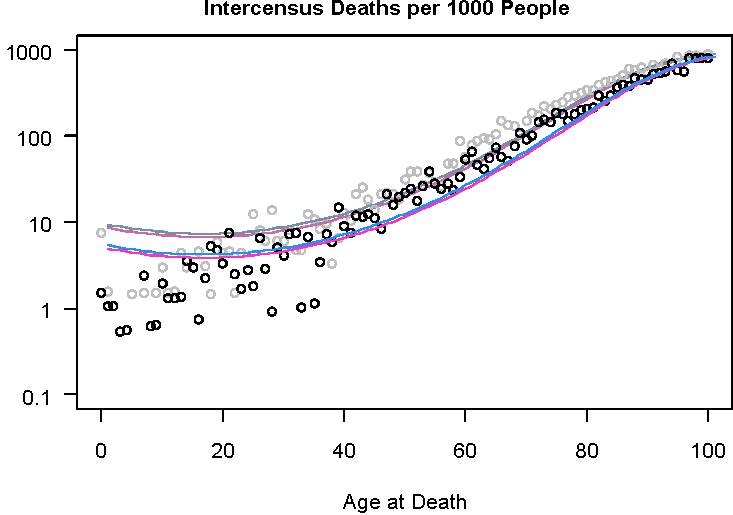
\includegraphics[scale=1]{figures/rtdice/mortality.pdf}
\caption{Fitted model $M_{4}$ plotted over the observed proportion of intercensus deaths per 1000 people by age.  For each of the 53 intercensus periods, Snoobs (black circles) die less frequently than non-Snoobs (gray circles), which reflected by the fitted lines as well.  Snoob women (bright pink) survive most frequently, closely followed by Snoob men (bright blue).  Non-Snoob men (dark blue) die most frequently of all, but at rates comparable to non-Snoob women (dark pink).}
\label{fig:mortality}
\end{center}
\end{figure}


% Table generated by Excel2LaTeX from sheet 'mort'
\begin{table}[htbp]
  \centering
  
    \begin{tabular}{llrrrrr}
    \hline
    \hline
    Model & Distribution & $k$     & AIC$_c$ weight & BIC weight & $\Delta$ AIC$_c$ & $\Delta$ BIC \\
    \hline
    $M_4$    & binomial & 5     & 100.00\% & 99.99\% & 0.00  & 0.00 \\
    $M_5$   & ZIB   & 7     & 0.00\% & 0.00\% & 20.41 & 39.87 \\
    $M_5$    & binomial & 6     & 0.00\% & 0.00\% & 21.20 & 30.94 \\
    $M_1$    & binomial & 2     & 0.00\% & 0.01\% & 47.62 & 18.41 \\
    $M_3$    & binomial & 4     & 0.00\% & 0.00\% & 49.82 & 40.08 \\
    $M_4$   & ZIB   & 6     & 0.00\% & 0.00\% & 76.98 & 86.71 \\
    $M_2$    & binomial & 3     & 0.00\% & 0.00\% & 122.52 & 103.05 \\
    $M_2$   & ZIB   & 4     & 0.00\% & 0.00\% & 309.24 & 299.50 \\
    $M_3$   & ZIB   & 5     & 0.00\% & 0.00\% & 717.33 & 717.33 \\
    $M_1$   & ZIB   & 3     & 0.00\% & 0.00\% & 1349.15 & 1329.68 \\
    $M_0$    & binomial & 1     & 0.00\% & 0.00\% & 15489.56 & 15450.62 \\
    $M_0$   & ZIB   & 2     & 0.00\% & 0.00\% & 15491.56 & 15462.36 \\
    \hline
    \end{tabular}%
    \caption{Model rankings for mortality models, with number of parameters ($k$).  To two decimal places, model $M_4$ completely dominates the information criterion weightings.}
  \label{tab:morttab}%
\end{table}%


\begin{table}[htbp]
  \centering
    \begin{tabular}{lcrrrr}
    \hline
    \hline
    Parameter & Estimate & Std. Error & 2.50\% & 97.50\% \\
    \hline
    $\alpha$    & 4.673 & 0.040 & 4.595 & 4.750 \\
    $\beta_1$    & -0.036 & 0.001 & -0.039 & -0.034 \\
    $\beta_2$    & -0.001 & 0.000 & -0.001 & -0.001 \\
    $\beta_3$    & -0.088 & 0.034 & -0.155 & -0.021 \\
    $\beta_4$    & 0.559 & 0.034 & 0.492 & 0.627 \\
    \hline
    \end{tabular}%
    \caption{Parameter estimates for model $M_{4}$ in a binomial model of mortality.  Snoob status substantially reduces the probability one will die at any given age or gender.} 
  \label{tab:m4ests}%
\end{table}%




\subsubsection{Mortality - What SnoobSim is Actually Doing}

Snoobs reference a different mortality schedule in the simulation specific to their age and gender.  The baseline mortality schedule for non-Snoobs is the estimated US mortality schedule c. 2005.  To be specific, the daily probability of death for each individual is calculated via:

\begin{verbatim}
daily.pr.death <- (1-(1/(1+exp(alpha + mortality.bias.male*male 
                                       + mortality.bias.snoob*snoob))))
\end{verbatim}

The parameter alpha represents the mortality schedule, but can be modified by both gender and Snoob status.  For this simulation, \texttt{mortality.bias.snoob} was set to -0.5, meaning Snoobs die less often, and and the \texttt{mortality.bias.male} was 0.3, meaning males die more often.  As a consequence, Snoobs should always die less for any given age and gender, and so the effects of this ``viability selection'' should show up in models that account for Snoob status.  



\subsection{SnoobSim Documentation}

SnoobSim is an agent-based population simulator in R that can be used to simulate virtually any demographic process in small populations.  It works by running through a daily list of stochastic events within the population and updating a master population register based on the outcome of these events, which can be influenced by the user.  Because population changes over decades, centuries, or longer can be simulated, a full record of every event inside the simulation is not intended to be saved.  Rather, the simulator records and exports census records taken in intervals specified by the researcher (e.g. every five years).  When it is time for another census, a copy of the population register for that day is saved, and when the simulation ends all such censuses are saved in csv format, as real field data would be stored.
  
Control of the simulator is managed through the ``control panel", a list of parameters at the top of the SnoobSim.r script.  These are divided into basic simulator values, such as the time between each census, initial population size, etc, vital population rates, such as age-specific fertility and mortality, etc. and evolutionary mechanisms, which control how the phenotypic traits of each individual are determined, and how they influence demographic parameters.  

Each day, the following demographic processes occur in this order:\\
1.	immigration \\
2.	births\\
3.	matings\\
4.	deaths\\
5.	emigration\\
6.	social learning / individual change\\

Since the simulation loops over days, which have relatively few births and deaths for realistic human populations, we expect that there are no important difficulties introduced by this order, or important differences if the order were changed.  

Immigration is controlled by two functions - \texttt{daily.immigration} and \\ \texttt{immigrant.maker}.  The first determines how many individuals will immigrate into the population that day, following the crude immigration rate specified by the user.  If there are indeed immigrants that day, the \texttt{immigrant.maker} function will create new entries in the population register for each of them. 

Mating occur only if there are fecund males and females.  Any female between 15 and 50 years old who is not currently pregnant can mate, as can any male between 15 and 60.  The \texttt{conception} function determines first if any women who can mate will actually do so that day; it determines this probabilistically by referencing an age-specific fertility schedule specified by the user.  Once it is determined that a female will become pregnant that day, the female will then choose an available male to be the father.  This is accomplished via the \texttt{mate.finder} function.  If no males are available then the woman will not become pregnant, but if at least one is available she will choose a male, each will count the other as their ``mate" in the population register, and the woman will become pregnant, beginning a daily countdown until birth saved to the ``counter" column in the population register.  The length of pregnancy here is approximately normal with mean 280 days and a standard deviation of 5 days.

Births only occur on days at which women reach the end of their pregnancy, as measured when the ``counter" column in the population register reaches 0.  For simplicity, women only given birth to one baby each pregnancy.  Each birth is added to the population through the \texttt{baby.maker} function.  

Deaths and emigrations occur in much the same manner.  For deaths, the\\ \texttt{grim.reaper} function probabilistically determines whether each individual in the population alive that day will die, as regulated by the age-specific mortality schedule set by the user.  Those individuals who die have their state variable in the population register changed from ``1" (alive) to ``0" (dead), and they play no further role in the demographic events of the population.  

For emigrants, the \texttt{daily.emigration} function determines how many, if any, individuals will leave the population that day, following the crude emigration rate set by the user.  Then, the \texttt{emigrant.picker} function will identify who is to leave, and sets their state from ``1" (alive) to ``11" (emigrated).  Individuals in the population register with a state of ``11" cannot participate in demographic events, but unlike the dead they are able to reenter the population as immigrants.  This aspect of immigration was not implemented, though.  

Provided individuals have not died or emigrated on a particular day, they then become available for individual change in their phenotypic characteristics.  One's Snoob status may be updated using a simple conformist heuristic.  Also, one's age measured in days increases by 1, as do the age-determined phenotypic characteristics of height and risk-taking score.   







